\section{RedoxOS}

\subsection{Nombre del proyecto o sistema operativo}

El sistema operativo examinado es "Redox OS". De acuerdo con \citep{redox_docs}, su denominación deriva de la palabra “Redox”, que es la abreviatura de “\textit{reduction–oxidation}”, un término de química que representa el intercambio equilibrado de electrones; esto refleja la meta del proyecto: alcanzar un sistema equilibrado en seguridad, rendimiento y simplicidad, a través de un diseño contemporáneo y fiable, redactado totalmente en Rust.

\subsection{Enlace al repositorio y/o documentación oficial}

\begin{itemize}
    \item \textbf{Enlace al repositorio oficial:} \url{https://github.com/redox-os} 
    \item \textbf{Enlace al libro oficial:} \url{https://doc.redox-os.org/book/}
\end{itemize}
\subsection{Objetivo del proyecto}
Según \citep{redox_docs, redox_github}, Redox OS tiene un enfoque fundamentalmente educativo y experimental, pero también pretende ofrecer una opción práctica y segura en comparación con sistemas Unix tradicionales. Su objetivo es probar que un sistema operativo que esté totalmente desarrollado en Rust puede lograr la misma estabilidad y eficiencia que los sistemas comerciales, mientras elimina categorías completas de errores relacionados con la memoria y la concurrencia.

\subsection{Lenguaje(s) de implementación}
Redox OS está predominantemente desarrollado en Rust, abarcando su kernel, controladores, gestor de memoria, sistema de archivos y gran parte de las herramientas de usuario.

Ciertos elementos específicos, como el cargador de arranque y aspectos de la compatibilidad con C, emplean "ensamblador y C" de manera restringida.

\subsection{Arquitectura del sistema }


Redox OS adopta una arquitectura híbrida de microkernel, inspirada en el diseño de Minix 3 y el modelo de Unix, pero con un enfoque mucho más fuerte en la seguridad y la modularidad.
El kernel de Redox es extremadamente pequeño: se encarga solo de la planificación, la gestión básica de memoria y la comunicación entre procesos.
Todos los servicios del sistema, como el manejo de archivos, controladores, red y entorno gráfico, se ejecutan en el espacio de usuario como procesos independientes llamados schemes.

\begin{figure}[H]
\centering
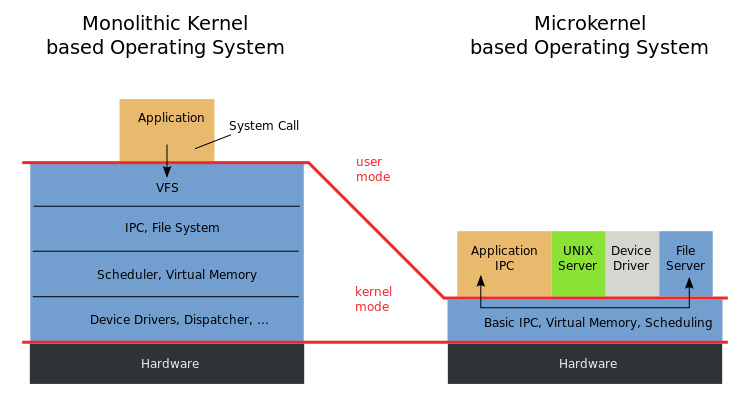
\includegraphics[width=1\textwidth]{figures/arquitectura.jpg}
\centering
\caption{Comparativa de la arquitectura de Redox frente a arquitecturas tradicionales.}
\label{fig:comparativaArquitecturaTheseus}
\centering
\small Fuente: Obtenido de \citep{redox_docs}.
\end{figure}


\subsection{Componentes implementados}

En Redox OS, los componentes principales del sistema se implementan como crates escritos en \texttt{Rust}, siguiendo una arquitectura microkernel. Cada crate encapsula un servicio o subsistema (procesos, memoria, sistema de archivos, E/S, etc.) con una estricta separación de privilegios.  
El microkernel se encarga de la comunicación por mensajes entre estos servicios, garantizando seguridad, aislamiento y estabilidad.  

A continuación, se presenta una tabla con los principales componentes y subsistemas de Redox OS, los nombres de sus crates en el repositorio oficial y la idea técnica detrás de su funcionamiento.

\begin{table}[H]
\centering
\caption{Funcionamiento técnico (idea clave) de los principales subsistemas de Redox OS}
\begin{tabular}{|p{5cm}|p{4cm}|p{6cm}|}
\hline
\textbf{Componente / Sub-sistema} & \textbf{Nombre en Redox (archivo/crate)} & \textbf{Funcionamiento técnico (idea clave)} \\ \hline
Gestión de memoria & \texttt{memory}, \texttt{paging}, \texttt{rmm} & Implementa paginación virtual por demanda y gestión de marcos físicos. \\ \hline
Gestión de procesos y multitarea & \texttt{kernel}, \texttt{scheme::proc} & Cada proceso se ejecuta en espacio de usuario, gestionado por el microkernel. \\ \hline
Sistema de archivos & \texttt{redoxfs} & Sistema de archivos nativo de Redox, implementado completamente en Rust. \\ \hline
Gestión de dispositivos y E/S & \texttt{drivers}, \texttt{schemes} & Controladores modulares gestionados como servicios de usuario schemes. \\ \hline
Comunicación entre procesos (IPC) & \texttt{syscall}, \texttt{scheme} & Utiliza el modelo \textit{scheme} para llamadas al sistema y paso de mensajes entre procesos y servicios del kernel. \\ \hline
Planificación y temporización & \texttt{scheduler}, \texttt{timer} & Planificador cooperativo basado en colas de prioridad. \\ \hline
Gestión de usuarios y permisos & \texttt{user}, \texttt{authd} & Módulos dedicados al control de autenticación y separación de privilegios mediante el servicio \texttt{authd}. \\ \hline
Interfaz gráfica (GUI) & \texttt{orbital}, \texttt{orbtk} & Entorno gráfico modular escrito en Rust; implementa servidor de ventanas y toolkit gráfico seguro. \\ \hline
Red y conectividad & \texttt{netstack}, \texttt{ethernetd}, \texttt{ipd} & Pila de red nativa en Rust, con servicios de capa física, IP y sockets; completamente en espacio de usuario. \\ \hline
Gestión del sistema y servicios & \texttt{init}, \texttt{logd}, \texttt{backgroundd} & Servicios del espacio de usuario que controlan inicialización, registros y tareas de sistema en segundo plano. \\ \hline
\end{tabular}
\centering
Fuente: Elaboración propia con base en \citep{ redox_github, redox_docs}.
\end{table}

\subsubsection*{Gestión de memoria}
La gestión de memoria es fundamental para el kernel de cualquier sistema operativo . Proporcionar una forma rápida de que los programas asignen y liberen memoria regularmente es una responsabilidad fundamental del kernel. Existen diversas implementaciones para asignar memoria física , como mapas de bits, asignación de amigos y el uso de estructuras de árbol o colas/pilas \citep{osdev_memory_management}.


\subsubsection*{Scheduling / multitarea}

Un scheduling algorithm determina cuánto tiempo de CPU se asigna a los procesos y subprocesos.  
El objetivo de cualquier algoritmo de planificación es cumplir con una serie de criterios fundamentales:

\begin{itemize}
    \item \textbf{Equidad:} ninguna tarea debe quedarse sin recursos; todas deben tener la oportunidad de usar tiempo de CPU.
    \item \textbf{Prioridad:} si se emplean niveles de prioridad, una tarea de baja prioridad no debe retrasar la ejecución de una tarea de alta prioridad.
    \item \textbf{Escalabilidad:} el planificador debe mantener un rendimiento estable ante un número creciente de tareas, idealmente con una complejidad de $O(1)$, como ocurre en el kernel de Linux.
\end{itemize}



\subsubsection*{Subsistemas de E/S y drivers}




\subsubsection*{Comunicación entre módulos}


\subsection{Herramientas utilizadas (compiladores, emuladores, etc.)}



\subsection{Nivel de complejidad y accesibilidad para estudiantes}